\subsection{PHY interface}

%\begin{figure}[ht]
%  \begin{center}
%    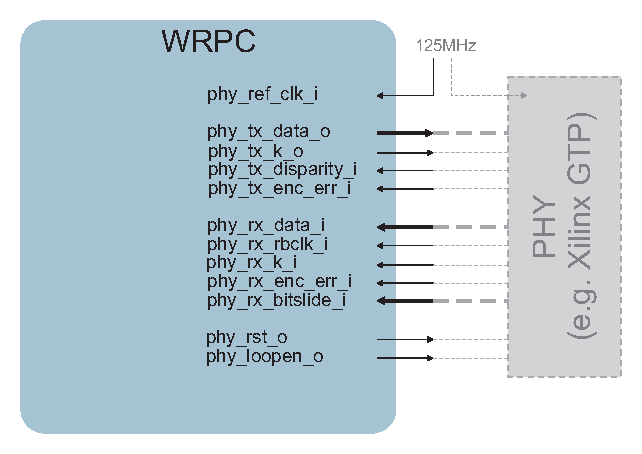
\includegraphics[width=.7\textwidth]{fig/wrpc_phyif.pdf}
%    \caption{PHY interface of WRPC}
%  \end{center}
%\end{figure}

The interface connects WRPC with the Ethernet PHY layer IP-core. The interface is generic, but
currently three Gigabit Ethernet PHYs are tested and supported:

\begin{enumerate}
\item Xilinx Spartan6 8-bit GTP SerDes
\item Xilinx Virtex6 16-bit GTX SerDes
\item Altera ``Deterministic Latency'' Transceiver PHY (tested on Arria V)
\end{enumerate}

Depending on the value of the \tts{g\_records\_for\_phy} and \tts{g\_pcs\_16bit} generic parameters,
WRPC expects to find the PHY signals in one of the following ports:

\begin{center}
  \begin{tabular}{|c|c|l|}
    \hline {\bf \tts{g\_records\_for\_phy}} & {\bf \tts{g\_pcs\_16bit}} & {\bf PHY ports}\\
    \hline
    \tts{false} & \tts{false} & \multirow{2}{*}{individual standard logic ports}\\
    \tts{false} & \tts{true} & \\
    \tts{true} & \tts{false} & \tts{phy8} record-based ports\\
    \tts{true} & \tts{true} & \tts{phy16} record-based ports\\
    \hline
  \end{tabular}
\end{center}

\begin{center}
  \fcolorbox{red}{white}{
    \parbox{.99\textwidth}{\textcolor{red}{\textbf{Important:}} If a WRPC user wants to use one of
      the supported PHYs, they have to be taken from the WRPC repository instead of manually
      generating them with the Xilinx/Altera tools. That is because WR developers have attached
      additional logic to them to improve their determinism. The easiest way of doing so is to make
      use of the provided Platform/Board Support Packages (see Sections~\ref{sec:hdl_platform}
      and~\ref{sec:hdl_board}).}}
\end{center}
